\section{Разработка средств симуляции и визуализации}
\label{sec:simulation}

В данном разделе будет произведен обзор средств симуляции работы оборудования а также средств визуализации данных, собранных дроном в процессе работы. Будет рассмотрен процесс дизайна и создания инструментов обработки данных, прошедших первичную обработу и восстановление облака точек, описывающего пространство, исследованное дроном.

\subsection{Общие сведения}
\label{sub:simulation:general}

Компонент для симуляции и визуализации состоит из двух основных частей. Первая часть - модуль симуляции полета дрона с возможностью установки различных параметров его положения в пространстве с помощью соответствующего API. Вторая часть - модуль работы с облаком точек а также софт для визуализации облака точек. Процесс взаимодейтсвия этого компонента с системами дрона таков:
\begin{itemize}
\item Дрон собирает информацию об окружении.
\item Компонент \textbf{TcpDroneUpdater} следит за дроном в реальном времени, проецируя его крен, тангаж и рысканье и ускорение на визуализационную модель.
\item Компонент \textbf{TcpCloudUpdater} следит за собранной дроном информацией и в реальном времени отображает облако точек, собранное дроном. Активация компонента опциональна и не всегда возможна ввиду большого количества данных, генерируемых дроном. Облако точек, генерируемое таким образом имеет пониженное разрешение.
\item После окончания сбора информации, вся собранная дроном информация (сохраненная на внутреннее хранилище) выгружается в софт визуализации, где из этих данных собирается полноразмерное облако точек.
\end{itemize}

Для упрощения процесса разработки инструментов и в виду не очень жестких требований к производительности данных инструментов, было принято решение разрабатывать инструментарий с применением языка C\# с последующим выполнением в среде \textbf{Mono} для Linux. В качестве фреймворка для визуализации трехмерных данных было принято решение использовать пакет Unity (Personal Edition) из-за его мультиплатформенности, простоты организации его компонентной модели а также возможности реализации логики визуализации на языке C\#, то есть возможности простой интеграции компонентов, считывающих данные о дроне в реальном времени с средствами визуализации.

\subsection{Симуляция полета дрона}
\label{sub:simulation:drone_simulation}
Для визуализации положения дрона в пространстве используются показания внутренних систем гироскопа, аккселерометра и компаса. Посредством беспроводной связи поисходит постоянная передача показаний этих сенсоров в виде следующих TCP-пакетов: 

\lstinputlisting[language={[Sharp]C}]{listings/RPYAccPacket.cs}

Поскольку симуляция использует Lock-step схему при передаче данных о положении дрона, решено использовать TCP соединение для избежания возможных рассинхронизаций положения/ориентации дрона внутри симуляции и в пространстве. Параметр Heading в данном случае является вспомогательным и калибровочным и позволяет установить связь между поворотом дрона и фактическим направлением его обзора.

\subsection{Обновление в реальном времени. Компонент TcpDroneUpdater}
\label{sub:simulation:realtime_updating}

Для сбора данных о положении дрона было решено использовать протокол TCP из-за Lockstep природы алгоритмов визуализации и их аппроксимационного характера в процессе сбора данных, когда происходит визуализация в реальном времени. Использование протокола TCP позволяет использовать встроенный в .NET тип TcpClient, позволяющий представить сетевой канал в виде потока данных (Порядок следования данных строго упорядочен пока соединение установлено, передача данных гарантируется). Пакет, будучи структурой фиксированной величины, можно обработать с помощью следующего компонента:

\lstinputlisting[language={[Sharp]C}]{listings/TcpDroneUpdater.cs}

Поскольку при использовании такого метода, задержка одного из пакетов либо скачки в показании приборов могут превести к внешним  ''рывкам'' при симуляции, на стороне контроллера объекта дрона реализованы алгоритмы линейной интерполяции данных параметров, так что ''промахи'' показаний датчиков практически не заметны.

\subsection{Визуализация облака точек}
\label{sub:simulation:point_cloud}
Вторая часть систем визуализации и симуляции - система отображения облака точек - служит для отображения данных, собранных дроном в процессе его работы. Для отображения точек используется специальный шейдер, позволяющий отображать только вершины mesh'а с опциональной возможностью изменения размеров и цвета отображаемых точек. Полученные mesh'ы могут содержать до десяти тысяч точек каждый. При достижении определенной плотности данных, облако точек можно использовать для восстановления трехмерной поверхности с адекватной точностью.

\begin{figure}[ht]
\centering
    \centering
    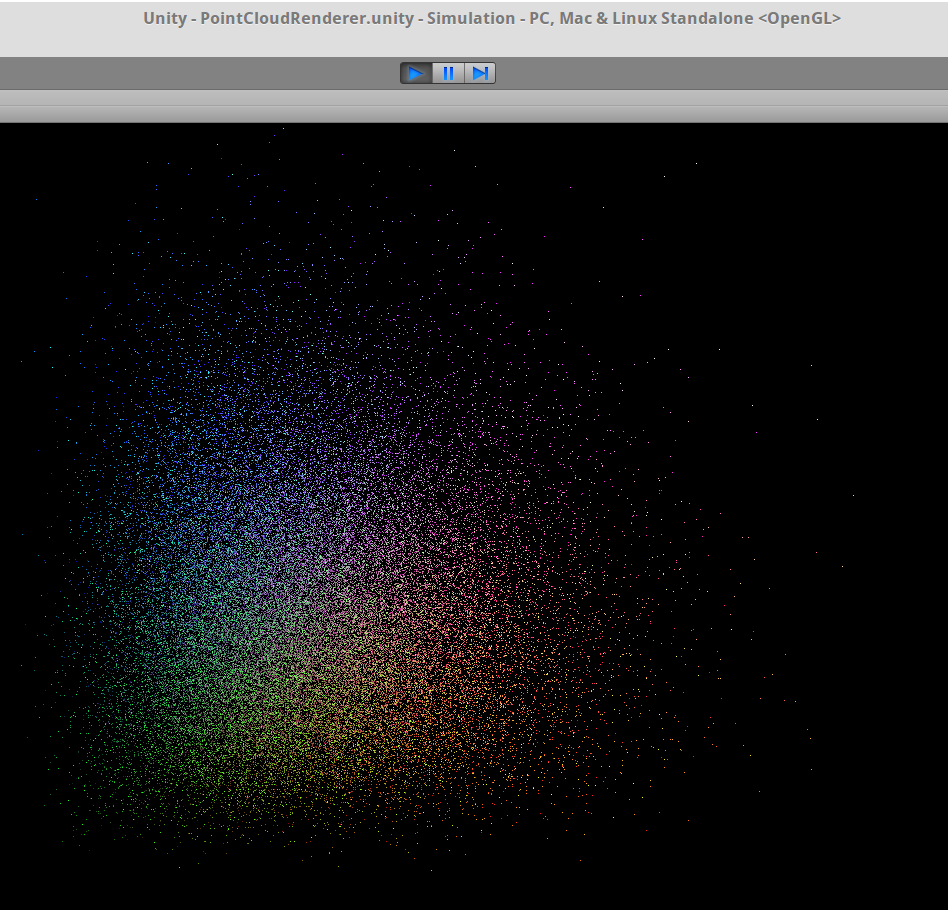
\includegraphics[scale = 0.4]{point_cloud.png}  
  \caption{Пример случайного облака точек с гауссовой плотностью распределением}
  \label{fig:point_cloud}
\end{figure}

Формирование точек для визуализации происходит по следующему алгоритму:
\begin{enumerate}
\item На вход алгоритма приходят двухмерные массивы-''кадры'' (frame) а так-же ассоциированное с кадром положение дрона в пространстве (описанная выше структура RPYAccPacket).
\item Расчитать поправочные коэффициенты xAdj, yAdj для вычисления угловых координат точек при проецировании на сферу вокруг дрона.
\item Для каждой точки в массиве frame
  \begin{enumerate}
  \item Умножить координаты (xi, yi) i-ой точки на соответствующие поправочные коэффициенты xAdj, yAdj.
  \item Провести луч из точки, находящейся между камерами дрона и направленного в направлении, соответствующем i-ому элементу массива..
  \item На расстоянии (1 - frame[xi, yi]) * Rсферы от камеры в направлении луча поставить точку и добавить ее на облако.
  \end{enumerate}
\end{enumerate}

Каждый кадр формирует свой набор точек, зависящий от положения дрона и содержимого массива frame. Для вычисления поправочных коэффициентов нужно учитывать такие параметры как угол обзора используемой камеры и разрешение изображения, передаваемого с камеры. Каждый элемент массива, являясь числом от 0 до 1 показывает удаление ассоциированной точки от камеры и зависит от радиуса сферы, на которую происходит проецирование точек. Так точки с нулевым значением показывают, что если предмет в них и находится, то он за пределами сферы, а значит на основе этой точки нельзя сделать точных выводов о расстоянии. (Ограничение радиуса сферы зависит в первую очередь от параметров аппаратной части не рассматривается в данной главе).

Поскольку отображение отдельных точек Mesh'а - нетипичная задача машинной графики, для отображения облака точек был разработан специальный шейдер (совместимый с Direct3D и OpenGL), чей листинг представлен ниже:

\lstinputlisting{listings/PointShader.shader}
